\documentclass[11pt]{article}
\usepackage{natbib}
\usepackage{fullpage}
\usepackage{draftwatermark}
\SetWatermarkText{DRAFT}
\SetWatermarkScale{5}
\title{\textbf{RenalQ draft - NZMJ paper}}
\author{Greig - introduction\\
		Iris / Jonathan - method\\
		Greig / Iris - results (1)\\
		Roger - results (2)\\
		Greig - discussion}
		\date{\today}

\usepackage{graphicx}
\begin{document}
\maketitle

%\tableofcontents

\section{Introduction}

This paper describes the development of an autonomous decision support tool for the interpretation of renal function tests. The tool provides clinicians with suggestions about the further management of a patient's test results. These suggestions are designed to be patient and context specific. The motivations behind the development of this application were to improve the quality of care patients that experience and to support the General Practitioner teams to manage the volume of results they receive on a daily basis. \\

An example was the discovery of an instance where a newly abnormal renal function result, in a patient who was acutely unwell. An experienced and caring physician had reviewed the latest renal function test result, making a clinical entry as the result's normality. This interpretation of the result did not seem to include the clinical context in which the test was requested or the patient's previous renal function test results. Despite the result being highly significant, the report did not generate any action until the patient represented several weeks later, stating that the patient informed the practice that they still felt unwell. Fortunately, this case ended well for the patient.\\ 

For any patient or condition, this is concerning but not uncommon, especially with regards to renal function test results.  As early management can change clinical outcomes, any missed test results are of concern. One study reported that American primary care physicians spent 74 minutes per day reviewing results. Despite which 81\% reported delays in managing results and only 41\% of clinicians were satisfied with their current process \citep{poon2004wish}. Estimates of "missed" or not followed up results vary from 6.8\% to 62\% \citep{callen2012failure}.\\

Another motivation was the rising incidence of chronic renal disease and the associated costs to society. The estimated Canadian prevalence of chronic renal disease in 2007-2009 was 12.5\% with 3.1\% of the population has grade 3-5 disease \citep{arora2013prevalence}. \citep{anachronistic}, described how despite the rising significance of renal disease worldwide, practitioner awareness remains low. These authors argued that care would need to be lead by primary care and integrated into general chronic condition management to avoid the "catastrophic" costs associated with the management of advanced chronic renal disease management \citep{jha2013chronic}. Kerr et al. estimated the cost of renal disease at 1.44-1-45 billion Pound Stirling in 2009-2010 for the UK alone \citep{underestimating}.\\

This paper will outline the development and implementation of the application. "RenalQ" was the final code name given to the product. The aim was to support the proactive management of renal disease by primary care clinicians. The methodology will describe how the application operated across the DHB but was able to consider each patient within their context.  Users described the application as making a positive change to their work processes, and many would like the methodology expanded to other tests. RenalQ was found to have a statistically significant impact on practitioner's' laboratory testing of renal disease, following its introduction.\\

\section{Method}

In the development of the RenalQ application a number of design decisions were made. It was decided that the RenalQ application would only provide decision support to the ultimately responsible clinician. This decision was entirely focused on patient safety. Compared to the treating clinician a decision support tool has access to only a finite subset of the total data set about a given patient which is available to the treating clinician. Information not available to the application may have significant and legitimate impact on the clinician's treatment decision.  The decision for the clinician to be the final arbitrator also acknowledges the possibility of error with a new developmental decision support application like "RenalQ". \\

The decision was also made to adopt industrial production methodology which has used statistical process control (SPC) as part of "business production management" \citep{rosemann2015six, cheng2015run, epprecht2015statistical}. This enabled the application to function at district scale, yet also be robust enough to consider the individual patient's needs. Within Health SPC has already been used to consider the operational function of emergency departments \citep{pimentel2015statistical} and the widest adoption of SPC in health has been within the field of quality improvement \citep{provost2011health}.\\

The resulting application is described in detail elsewhere\citep{GodfreyEtAl2014KidneyPaper}. In essence RenalQ interprets the eGFR result for each patient, within the context of their previous eGFR results. In the laboratory work flows, RenalQ is executed only after the usual renal function tests have been performed and assuming it is appropriate to calculate the eGFR has been calculated by the usual laboratory processes. If the patient is deemed to be acutely unwell, the eGFR algorithm is not applicable and so neither it or RenalQ is executed.\\

The RenalQ interpretation engine consists of three layers depending on the number of eGFR results available within the laboratory database. If the patient has less than five results no specific advice is given. Between 5-19 results the eGFR is interpreted by a set of fixed heuristics rules. These encode standard clinical practice, but with two bias being introduced. The first bias is that result returned by the application to the treating clinician would be clinically conservative and encourage clinician to be proactive in their care of the patient. The second bias introduced was that RenalQ encouraged further testing to improve its own accuracy. The first bias is aimed to provide clinical safety. We accepted that it might be unnecessarily alarmist on occasions but in the balance between irritating users against maintaining patient safety, the decision was made to prioritize patient safety. The third layer in RenalQ applied for patients in whom 20 or more test results were available and used SPC to provide an interpretation. This layer used cumulative summation as the SPC methodology to determine changes in the recent past away from the historic usual pattern for this particular patient. On the basis of the rate of change interpretations and suggestions were developed. The second layer in the interpretation engine was found to be critically important for the ability of RenalQ to reliably detect acute renal failure. This rule was called the "plummet" rule for the rate of deterioration in the eGFR from previous levels for obvious reasons. \\

There was a body of work beyond the scope of this practice around integration of the RenalQ application into the laboratory computer systems. There was a degree of technical complexity required to resolve transfer of data between the laboratory systems and RenalQ, then for the RenalQ interpretations to be made available to Primary Care within the usual results of the renal function tests. Like all such technical exercises, a lot of work was required to make it look like nothing special had occurred. \\

Once the application was operationally ready for evaluation by primary care providers, ethical approval for the trial to proceed gained from the Hospital and Community Clinical Boards. \\

\section{Evaluation}

Evaluating RenalQ was performed iteratively through three phases. The first phase was pre-deployment where the evaluation was focused on optimizing of the interpretation engine. A series of progressively larger samples of deidentified historic renal function results was obtained from the laboratory. The suggestions from RenalQ were manually compared to the interpretations of an experienced clinician. Initially frequent improvements to the algorithm were required, particularly around the identification of acute renal impairment. 

Once the algorithm was adjusted, it became clear that sensitivity was over 99\% specificity was over 98\%. this high level of sensitivity and specificity created its own problems. It was easy to slip into the trap during this phase of the evaluation that because RenalQ was usually accurate, it became the source of truth for its own evaluation. The question of RenalQ's accuracy became quickly begged! To balance this tendency, the results of RenalQ were reviewed by the local renal physicians to ensure selectivity and specificity were progressively optimised. As a group they were comfortable with the interpretations provided by RenalQ as being safe and appropriate for a pilot study. \\ 

The third phase of RenalQ's evaluation was both qualitative and quantitative. The qualitative evaluation was performed during the limited pilot study and through into the initial period following the launch of the application into an extended pilot. 

A semi-structured responsive interview instrument was used as this was seen as an ideal way to allow primary care staff to reflect on their experiences with RenalQ allowing them to provide in-depth feedback. In a responsive interview the emphasis is on the fact that the interviewer and interviewee are both people and that they form a relationship during the interview \citep{rubin2011qualitative}. Additionally, the research design is able to remain flexible throughout the project meaning that if new information, or a new area of interest, is uncovered then the current interview, and subsequent interviews, can probe this area. It allows the concept of ‘we don’t know everything’ to be included in the research design.\\

Validity concerns the "believability" of a statement and is a characteristic given to a claim by those to whom the claim is addressed. Validity in qualitative research is seen as an activity that is conducted throughout the research process \citep{morse2002verification, kvale2009interviews} to convince readers of the likelihood that the support for the claim is strong enough to serve as a basis for understanding \citep{polkinghorne2007validity}. Throughout the process it was the views of primary care staff that were sought, listened to, and clarified where meaning was not understood. The result of the process is that the research reflects the primary care view of RenalQ and not that of the researcher.\\

A series of interviews of individual clinicians and groups were undertaken. Where interviews were conducted, the semi structured responsive interview process was followed. Where a large group was encountered the approach was altered into a focus group approach based on the semi-structured questions.\\

At each event there was a clear message that RenalQ added value to general practice. Reflective comments from GP included - “don’t take it away” and a “really useful tool”. After only a relatively short period of time the GP interviewed appeared to place confidence on the RenalQ interpretation and this both “sharpened their practice” and “saved time”\\

RenalQ was felt to save time, in contrast to the fear it would increase GP workload. The GP perspective on this aspect was that the RenalQ interpretation provided an additional check giving them confidence in their proposed action. In part this was due to the believe that the sensitivity of RenalQ with respect to its interpretations was set correctly. Feedback received indicated that although RenalQ was seen as conservative in its interpretations, this was considered to be appropriate. In this regard the overall feeling was that the interpretation was seen as more reliable.\\

The General Practitioners felt the RenalQ process should be applied to outpatient renal function tests from the hospital as well as community requested samples. This anomaly was due the laboratory deeming all hospital samples to be taken from patients not in their steady state, not just those acutely unwell. General Practitioners also requested the methodology be extended to other areas of laboratory result interpretation.

We limit our investigation of the total amount of testing being conducted to the last 39 months from January 2013 to March 2016.\\

\begin{figure}[htp]
\centering
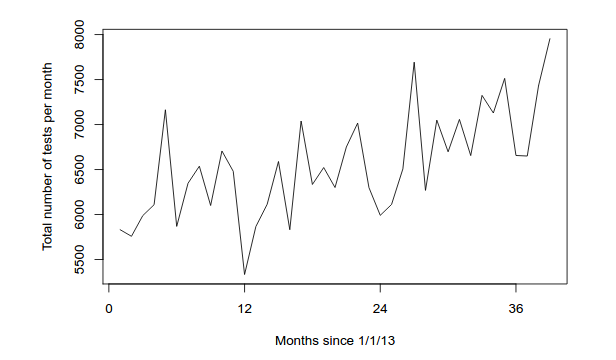
\includegraphics[scale=0.50]{Fig1.png}
\caption{}
\label{}
\end{figure}

There is a (perhaps not so obvious) pattern in this data to draw to the reader's attention. It seems both a seasonal effect over the months within a year, and a general increase over years should be noted.  Our belief in this notion is supported by use of an Analysis of Variance (ANOVA) procedure. \\

\begin{figure}[htp]
\centering
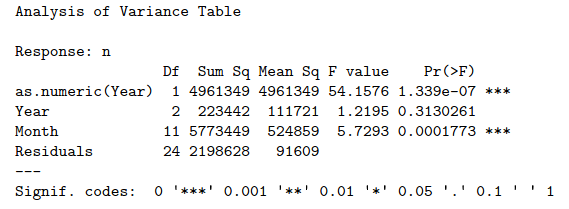
\includegraphics[scale=0.50]{fig2.png}
\caption{}
\label{}
\end{figure}

The above table (figure 2) shows that the impact of year can be summarised as a straight line effect, while we have a cyclic pattern over the months. Any departure from this would constitute an unusual increase in total workload since the introduction of RenalQ. We use a standard control chart for individuals to search for unusual results. The control limits on the plot are calculated using the data from before the introduction of RenalQ and are at two (shown in orange) and three (shown in red) standard deviations from the centre line (see figure 3).\\

\begin{figure}[htp]
\centering
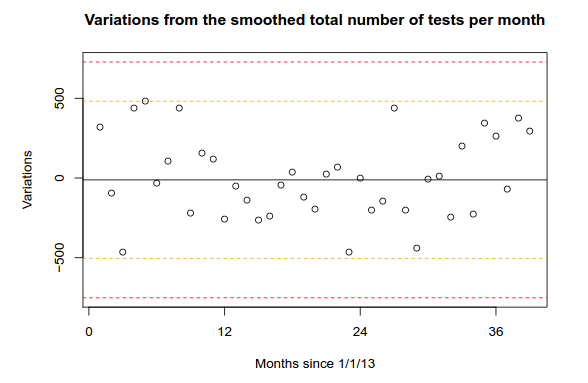
\includegraphics[scale=0.50]{fig4.png}
\caption{}
\label{}
\end{figure}

There are no serious  departures (outside three standard deviation limits) from what could be expected in terms of the total number of tests being conducted. We do need to condition this assessment on our concern that the totality of tests has not been provided for earlier years of this investigation. This aspect of this report can be re-created once the reliability of the complete data can be established.\\

Even though the total number of tests is growing, it is worth seeing if the mix of tests is changing at all. We have used a $\chi^2$ test to see if the counts of tests yielding different eGFR values is changing over time. The eGFR values have been put into five categories using cut-offs of 15, 30, 60, and 90\\

\begin{figure}[htp]
\centering
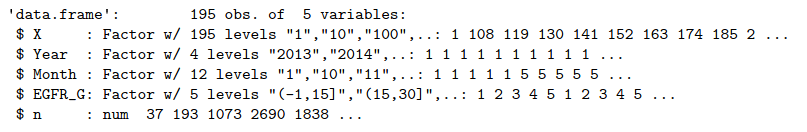
\includegraphics[scale=0.50]{fig5.png}
\caption{}
\label{}
\end{figure}

The test has a $\chi^2$ value of 3175.89 (p=0, df=152) which means there is a change in the pattern of testing over time for the five categories.\\

\begin{figure}[htp]
\centering
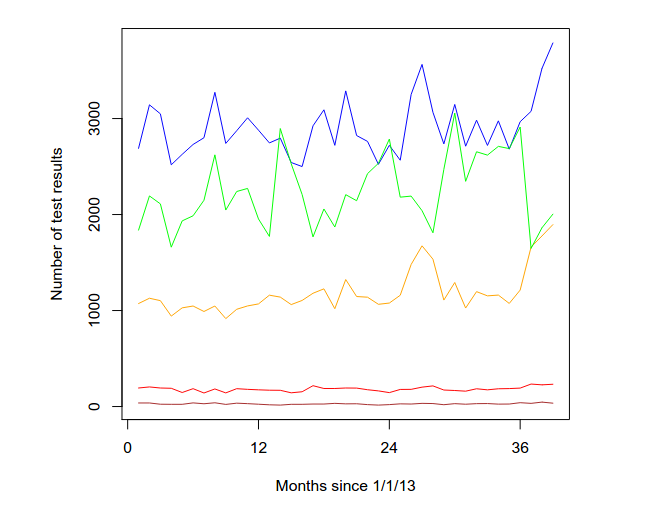
\includegraphics[scale=0.50]{fig6.png}
\caption{}
\label{}
\end{figure}

It is difficult to see any growth in the number of tests being conducted for patients whose eGFR is between 60 and 90 (shown in blue) and above 90 (shown in green). The patient groups of greatest interest are those with eGFR between 30 and 60 (shown in orange) and between 15 and 30 (shown in red).\\

In the following analysis, the data for 2013 has been added back in and we have evaluated every value of eGFR instead of grouped eGFR values.The next  model  used to identify the statistically significant factors affecting the time between successive renal function tests allows for only the level of renal function for each patient (as measured by their eGFR), and whether that test was analyzed using the RenalQ system. In addition, the combination of these two effects has also been incorporated in the model. The regression model for this model yields  the following summary of effects and their statistical significance. \\

\begin{figure}[htp]
\centering
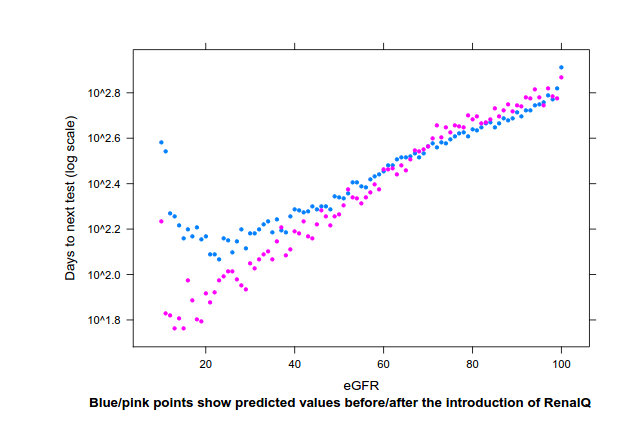
\includegraphics[scale=0.50]{FigCritical.png}
\caption{}
\label{}
\end{figure}

\section{Conclusions}
The management of laboratory results in general and the management of renal disease are both significant issues. The combination of an aging population and an increasing incidence of predisposing illness such as diabetes means renal disease will become even more significant in the future. For the practitioner, renal function tests needs to be interpreted within the patient's context. The same result will mean different things in different patients. With time frames for chronic renal impairment being measured in months or years, losing contextual awareness of the significance and interpretation of any one result in a busy practice borders on the inevitable. Yet the consequences for both the patient and the affordability of health care is significant.\\

RenalQ is the first generation of "SMART" solutions to these types of clinical problems. By providing individualized, situational assistance to the clinician at the point of decision making, the clinician is given more opportunity to make the right decision for the particular patient. This is independent of whether the clinician agrees with RenalQ or not. The result was flagged as one about which a decision needed to be made.\\ 

As a quality improvement activity RenalQ has been effective. RenalQ would have flagged the original missed test results as being significant. On a district scale it has provided this level of support to every patient of every practitioner. RenalQ has demonstrated that it decreases the time between sequential renal function tests for those patients who are most at risk of progressing to requiring dialysis. \\

As an innovation methodology the development of RenalQ took only four years from conceptualization to being able to demonstrate statistically significant patient benefit. Typically the time frame for the successful implementation of effective innovation into clinical practice is 17 years \citep{morris2011answer}. Being the author's first project there was a steep learning. Equally having traversed the learning curve once, the next application should have an even shorter time frame than four years from conceptualization to delivering clinical benefits. \\

Part of the success of this project was due to the use of the R statistical language \citep{rstat2013}. This powerful and effective language for data analysis leading to both insight and new products is a New Zealand success story. Developed by Ross Ihaka and Robert Gentleman from the University of Auckland and first released in 1994, R language now features in lists of the top ten languages used in the world. Almost unbelievably, R statistical language was developed and is maintained as an open source project that is free to use across multiple platforms. Given the explosion in the quantity of data collected, the need for smart use of resources but the development needs to occur within a tight fiscal envelope, R statistical language represents a compelling option for future developments. \\



\bibliographystyle{plain}
\bibliography{NZMJ}

\end{document}
